\documentclass[conference]{IEEEtran}
\IEEEoverridecommandlockouts
\usepackage{cite}
\usepackage{amsmath,amssymb}
\usepackage{graphicx}
\usepackage{booktabs}
\usepackage{xcolor}
\usepackage{placeins} % \FloatBarrier keeps all figures before the references
\usepackage[hidelinks]{hyperref}
\graphicspath{{figures/}}
\renewcommand{\topfraction}{0.9}
\renewcommand{\dbltopfraction}{0.9}
\renewcommand{\textfraction}{0.07}
\renewcommand{\floatpagefraction}{0.8}
\renewcommand{\dblfloatpagefraction}{0.8}

\begin{document}

\title{Calibration Budgets Do Not Transport Across P300 Speller Protocols: A Cross-Cohort Analysis of bigP3BCI}

\author{\IEEEauthorblockN{Devansh Sati}
\IEEEauthorblockA{\textit{Department / Institution} \\
\textit{City, Country} \\
devanshjsati@gmail.com}}

\maketitle

\begin{abstract}
P300 spellers need subject-specific calibration before use, and methods that shorten calibration are usually validated on a single dataset. We asked whether the calibration budget a P300 speller needs is a stable property of the decoder or varies across recording protocols and cohorts. Using 14 eligible cohorts of the public bigP3BCI archive (224 participants, 566 records), we trained a fixed shrinkage-LDA decoder on the first $k$ calibration characters in recording order and decoded all test characters offline. The budget B80 is defined as the smallest $k$ at which 80\% of a cohort's participants reach 70\% character accuracy. We estimated B80 where offline decoding reproduced online accuracy, and a co-primary budget based on flash-level AUC $\geq 0.75$ in all cohorts. Budgets ranged from 2 to 30 characters, a 15-fold spread under both definitions and a 10--18-fold spread across ten robustness variants. Learning-curve slopes were heterogeneous ($I^2=0.88$). No single budget brought 80\% of all participants to usable accuracy, and a budget borrowed from other cohorts missed a withheld cohort's budget by at least two characters in every cohort (median error 12--13 characters). Pre-specified protocol descriptors did not explain the differences; in an exploratory analysis, artefact rejection rate was associated with slower learning (Holm-corrected $p=0.016$). A calibration length validated on one P300 dataset should not be reused on another; budgets should be set per protocol and site and reported with recording quality.
\end{abstract}

\begin{IEEEkeywords}
brain--computer interface, P300 speller, EEG, machine learning, sample efficiency, dataset shift, calibration, reproducibility
\end{IEEEkeywords}

\section{Introduction}
P300 spellers let people with severe motor impairment, including amyotrophic lateral sclerosis (ALS), communicate by attending to flashing characters \cite{farwell1988,sellers2006}. Each new user must first copy-spell while labelled EEG trains a classifier. Calibration costs time and adds fatigue, and a minority of users never reach usable control at all \cite{guger2009}, so shortening calibration is a central goal of the field.

Most work proposes a method and shows that it needs less calibration on one dataset. Self-supervised pretraining with P300 aggregation, for example, was reported to cut calibration by 60\% on BCI Competition II-B \cite{hong2025}; transfer and semi-supervised methods make similar single-dataset claims \cite{gao2023,chen2026,wu2022}. A budget found sufficient in one setting is then implicitly treated as sufficient elsewhere, although P300 protocols differ in grid size, flash paradigm, timing, electrodes, test procedure and population.

Gorenshtein et al.\ recently showed on bigP3BCI that the mapping from calibration-data quality to online accuracy does not transport across cohorts \cite{gorenshtein2026}. Their analysis always used the full calibration block, which leaves open how \emph{much} calibration is needed and whether that amount transports. In machine-learning terms, calibration size is the number of labelled training examples a subject-specific classifier receives, so the question is one of sample efficiency under dataset shift: does a classifier's learning curve \cite{viering2023}, and hence its required training-set size, generalise across data-generating conditions, a concern that distribution-shift benchmarks have made central in machine learning \cite{koh2021}? We address this question. Our contributions are: (i) calibration learning curves for a fixed reference decoder in 14 cohorts, with calibration truncated strictly in recording order; (ii) per-cohort budgets based on character accuracy and on test-length-independent AUC, with bootstrap intervals; (iii) estimates of between-cohort heterogeneity, its moderators and leave-one-cohort-out transportability; and (iv) open code that reproduces every result.

\section{Related Work}
\subsection{Reducing calibration}
Approaches include subject-independent and self-trained CNNs \cite{gao2023}, semi-supervised adaptation \cite{chen2026}, self-supervised pretraining \cite{hong2025} source-sample selection for transfer \cite{kilani2024}, and EEG foundation models pretrained on large multi-dataset corpora \cite{jiang2024}; transfer learning for EEG has been reviewed in \cite{wu2022}. Each is evaluated on one or a few datasets, and none measures how the required budget varies across protocols.

\subsection{Cross-dataset P300 analysis}
MOABB benchmarks ERP pipelines at a fixed training size \cite{moabb2024}; signal alignment improves classifier transfer across P300 datasets \cite{song2024}; and merging public P300 datasets has been discussed \cite{bianchi2022}. These works concern classifier transfer, not the subject-specific calibration a new cohort needs.

\subsection{Predicting performance from calibration}
Detectability indices predict P300 speller accuracy within a study \cite{mainsah2016}. Gorenshtein et al.\ found such mappings to be cohort-specific \cite{gorenshtein2026}. They asked whether a calibration \emph{score} transports; we ask whether a calibration \emph{budget} does.

\section{Data}
\subsection{Archive}
We used bigP3BCI v1.0.0 \cite{bigp3bci}: 20 visual P300 speller studies recorded in BCI2000 \cite{schalk2004} at Duke University and East Tennessee State University, comprising 6{,}980 EDF+ files with a shared 16-channel montage at 256\,Hz. Each session has a calibration (Train) phase without feedback and a Test phase with online feedback. Per-character flag channels record which characters each flash lit, which allows character decoding for every flash paradigm, including row--column and checkerboard layouts \cite{townsend2010}.

\subsection{Eligibility}
The unit of analysis is a participant\,$\times$\,session\,$\times$\,condition record with its own Train and Test files. Studies C and P were excluded because their online outcomes cannot be recovered \cite{gorenshtein2026}. Studies D, F, G and H were excluded because calibration and testing were recorded in different conditions. Cohorts with at least 5 participants and 4 evaluable budget levels were eligible, giving 14 cohorts (Table~\ref{tab:cohorts}).

\begin{table}[!tb]
\centering
\caption{Eligible cohorts. Acc.: character accuracy at full calibration (offline / online). Rej.: share of calibration epochs $>150\,\mu$V. \checkmark: offline within 0.10 of online.}
\label{tab:cohorts}
\setlength{\tabcolsep}{3pt}
\footnotesize
\begin{tabular}{lrrrrrcc}
\toprule
Cohort & $N$ & Rec. & Grid & ISI & Rej. & Acc. & Valid\\
\midrule
A & 13 & 39 & 72 & 125 & .00 & .82/.79 & \checkmark\\
B (ALS) & 18 & 56 & 36 & 250 & .01 & .92/.90 & \checkmark\\
E & 8 & 8 & 72 & 125 & .00 & .80/.92 & \\
I & 13 & 26 & 72 & 125 & .23 & .47/.65 & \\
J & 20 & 40 & 36 & 125 & .35 & .43/.70 & \\
K & 5 & 16 & 72 & 125 & .61 & .29/.75 & \\
L (ALS) & 11 & 33 & 36 & 250 & .00 & .86/.84 & \checkmark\\
M & 21 & 42 & 72 & 125 & .26 & .54/.82 & \\
N (ALS) & 8 & 16 & 36 & 250 & .21 & .63/.69 & \checkmark\\
O & 17 & 34 & 72 & 125 & .01 & .91/.88 & \checkmark\\
Q & 36 & 108 & 72 & 125 & .01 & .83/.83 & \checkmark\\
R & 20 & 80 & 72 & 188 & .01 & .97/.96 & \checkmark\\
S1 & 10 & 20 & 72 & 188 & .00 & 1.00/1.00 & \checkmark\\
S2 & 24 & 48 & 72 & 188 & .00 & .97/.98 & \checkmark\\
\midrule
Total & 224 & 566 & & & & & 9\\
\bottomrule
\end{tabular}
\end{table}

\begin{figure*}[!t]
\centering
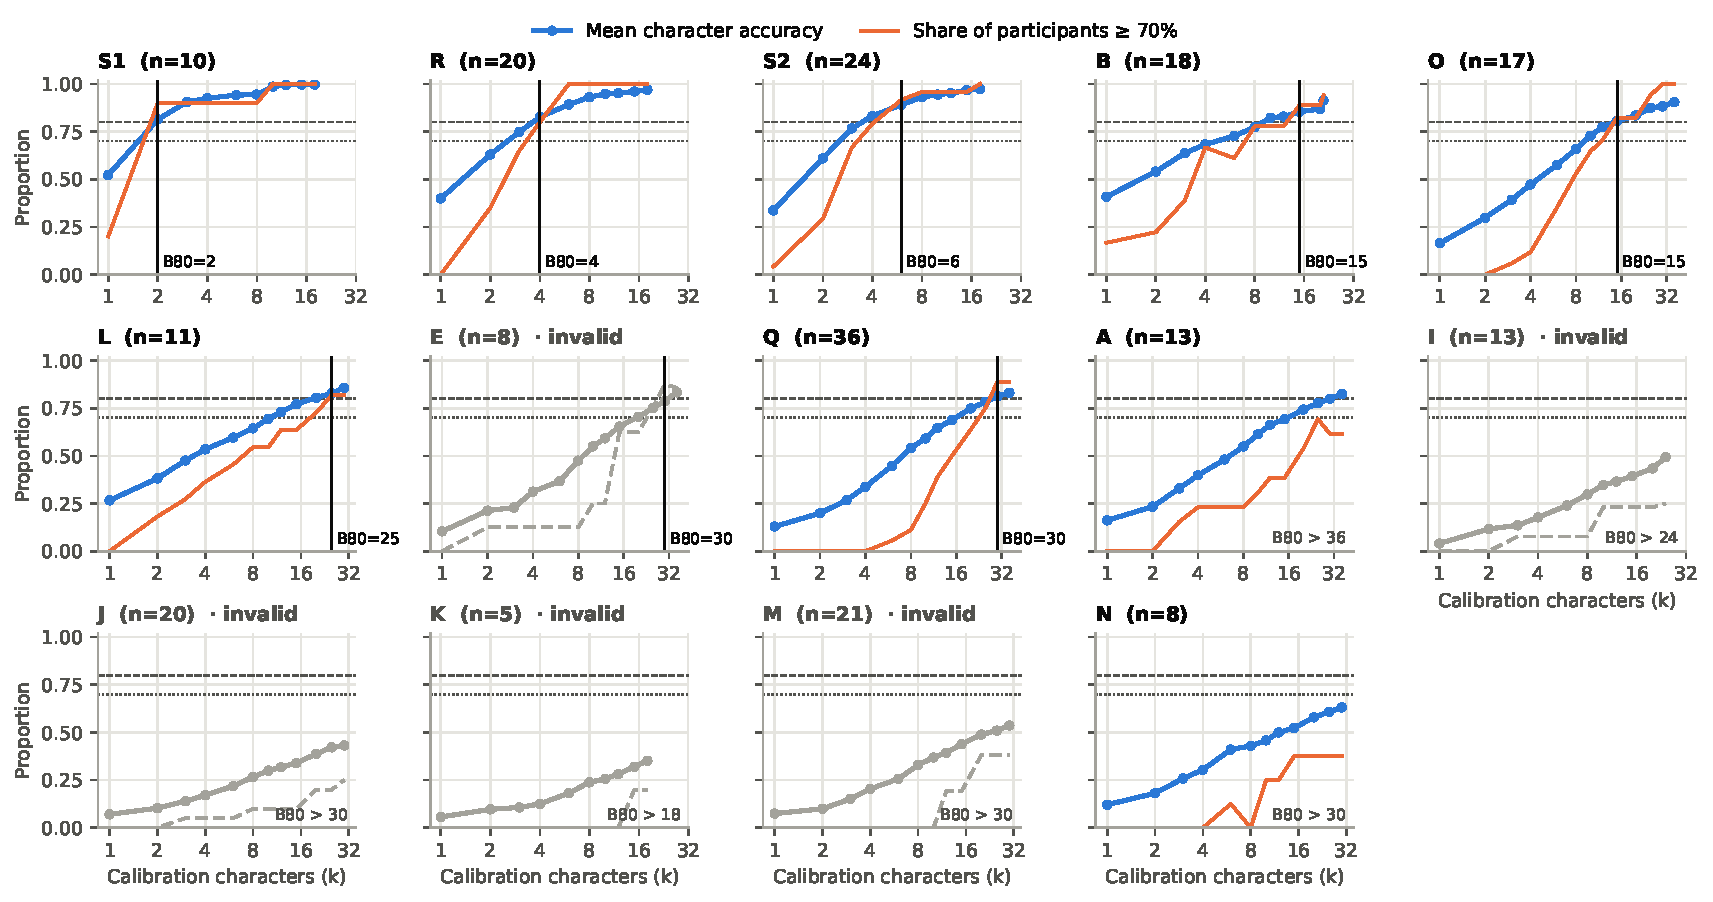
\includegraphics[width=\textwidth]{fig1_learning_curves_paper.pdf}
\caption{Calibration learning curves per cohort: mean character accuracy (blue) and share of participants at $\geq 70\%$ (orange) versus calibration characters $k$. Vertical line: B80. Grey panels: offline decoding not valid (dynamic-stopping tests).}
\label{fig:curves}
\end{figure*}

\section{Methods}
\subsection{Preprocessing}
The 16 shared channels were band-pass filtered (0.5--30\,Hz, 4th-order zero-phase Butterworth) and epoched from $-200$ to 800\,ms around each flash. Epochs were baseline-corrected and decimated to 64\,Hz, giving 832 features per epoch. Calibration epochs exceeding 150\,$\mu$V were excluded from training; test epochs were decoded as recorded. All analysis settings were fixed in a configuration file before the full run, and none was tuned on test data. EDF files were read with MNE-Python \cite{gramfort2013}, filtering used SciPy \cite{virtanen2020}, classification used scikit-learn \cite{pedregosa2011}, and statistical models used statsmodels \cite{seabold2010}.

\subsection{Machine-learning formulation}
Each flash yields a feature vector $\mathbf{x}\in\mathbb{R}^{832}$ (16 channels $\times$ 52 samples) and a label $y\in\{0,1\}$ (target or non-target), giving a binary classification problem with class imbalance from 1:3 to 1:11 (target rate 8--25\% across cohorts). Features are standardised using calibration statistics only. We use shrinkage linear discriminant analysis, the standard P300 classifier \cite{blankertz2011}, which scores a flash as
\begin{equation}
s(\mathbf{x})=\mathbf{w}^{\top}\mathbf{x}+b,\qquad \mathbf{w}=\hat{\Sigma}_{\lambda}^{-1}(\hat{\boldsymbol\mu}_1-\hat{\boldsymbol\mu}_0),
\end{equation}
where $\hat{\boldsymbol\mu}_c$ are class means and the covariance is shrunk towards a scaled identity,
\begin{equation}
\hat{\Sigma}_{\lambda}=(1-\lambda)\,\mathbf{S}+\lambda\,\nu\mathbf{I},\qquad \nu=\operatorname{tr}(\mathbf{S})/d,
\end{equation}
with $\lambda$ chosen analytically by the Ledoit--Wolf estimator \cite{ledoit2004}. Shrinkage keeps $\hat{\Sigma}_{\lambda}$ well conditioned when the number of training epochs is small relative to $d=832$, which is exactly the low-calibration regime studied here; no hyperparameter is tuned per subject or cohort.

\textit{Character inference.} A test character is spelled with a sequence of flashes $\mathcal{F}$; let $\mathcal{F}_c\subseteq\mathcal{F}$ be the flashes that lit candidate character $c$. The decoded character is
\begin{equation}
\hat{c}=\arg\max_{c}\ \frac{1}{|\mathcal{F}_c|}\sum_{f\in\mathcal{F}_c}s(\mathbf{x}_f),
\end{equation}
using all flashes the original protocol presented. The mean (rather than sum) makes the rule valid for checkerboard paradigms, where characters are lit unequally often.

\textit{Learning curves.} For each record and each training-set size $k\in\{1,2,3,4,6,8,10,12,15,20,25,30,\dots,\text{full}\}$ calibration characters, the classifier is trained only on the first $k$ characters in recording order (72--180 epochs per character, median 120), so smaller training sets are strict subsets of larger ones and evaluation never uses calibration data. This yields 7{,}050 trained models across 566 records, i.e.\ an empirical learning curve per record \cite{viering2023}.

\textit{Controls and verification.} A label-permutation control (shuffled calibration labels) gave chance-level accuracy in every cohort (at most 0.01 above chance), and real labels exceeded it by at least 0.28. With full calibration, offline accuracy reproduced the original online accuracy in pilot sessions (0.94 vs.\ 0.92; 0.93 vs.\ 0.93). An independent re-implementation of truncation, training and decoding, written separately from the pipeline, reproduced the accuracy of randomly sampled records at all budgets exactly (maximum difference $10^{-16}$), found no test epoch in any calibration set, and recomputed every budget identically.

\subsection{Calibration budgets}
Participant accuracy at $k$ was pooled over that participant's records. A budget $k$ was evaluable when at least 80\% of a cohort's participants had data at $k$. B80 is the smallest evaluable $k$ at which at least 80\% of participants reach 70\% character accuracy, right-censored if none qualifies. In five cohorts (E, I, J, K, M), tests used dynamic stopping \cite{mainsah2015} and offline accuracy fell more than 0.10 below online accuracy, so B80 is interpreted in the 9 cohorts with valid decoding. This restriction was decided after inspecting full-calibration accuracy; including all 14 cohorts leaves the B80 range unchanged (2--30 characters), because E reaches B80 at 30 and I, J, K, M are censored. The co-primary AUC budget applies the same rule to flash-level AUC $\geq 0.75$, which does not depend on test length, in all 14 cohorts. Intervals came from 2{,}000 participant-cluster bootstrap resamples.

\subsection{Statistical analysis}
Stage~1 fitted, per cohort, a binomial GLM of correct characters on $\log k$ (or OLS of AUC on $\log k$), centred at $k=4$, with participant-clustered standard errors. Stage~2 pooled cohort slopes and intercepts with DerSimonian--Laird random effects \cite{dersimonian1986}, reporting $\tau$, $I^2$ \cite{higgins2002}, a Hartung--Knapp confidence interval and a prediction interval. Seven pre-specified protocol descriptors (seconds per calibration character, test flashes per character, grid size, inter-stimulus interval, row--column share, characters lit per flash, ALS cohort) entered one at a time in a Knapp--Hartung meta-regression of slopes \cite{knapp2003}. Artefact rejection rate was added afterwards as an exploratory descriptor, motivated by the high rejection rates in the cohorts that never reached a budget; Holm correction \cite{holm1979} was applied across all eight. For transportability, each cohort was withheld in turn and its budget predicted from the remaining cohorts' pooled participants (primary) or from the median of their budgets (secondary). The stage-2 code recovered a known moderator effect, and no spurious one, on simulated data.

\section{Results}
\begin{figure}[!tb]
\centering
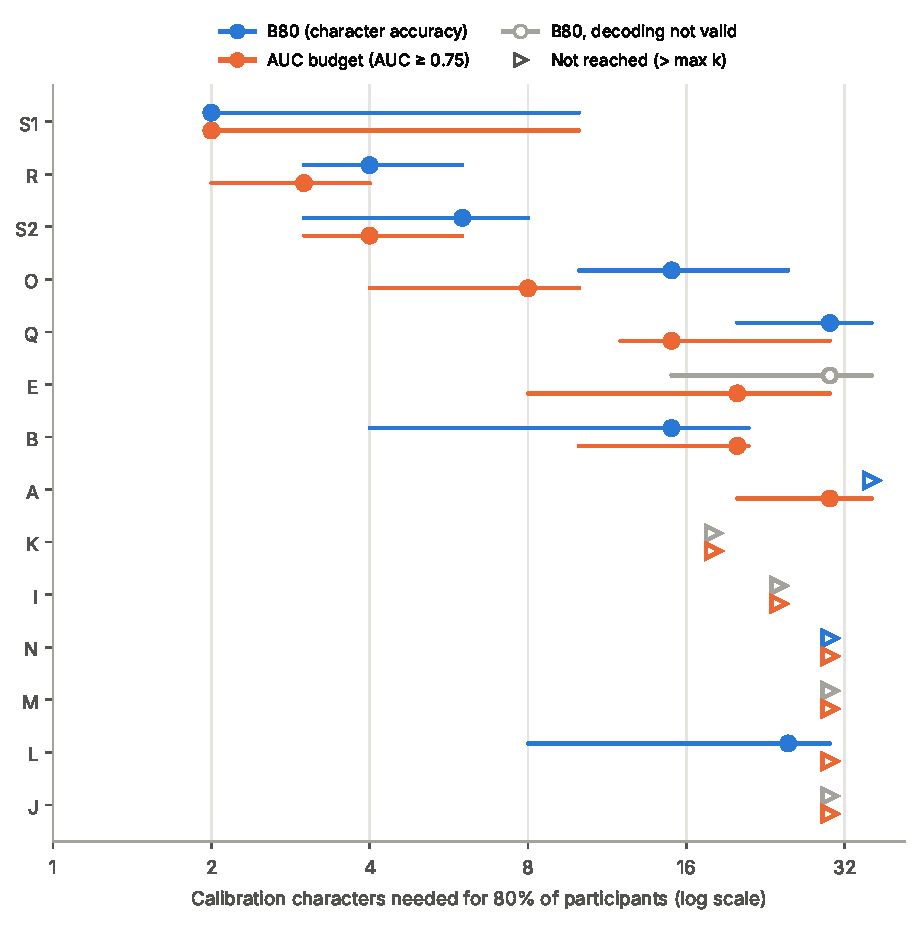
\includegraphics[width=\columnwidth]{fig2_budgets_paper.pdf}
\caption{Calibration budget per cohort: B80 (blue) and AUC budget (orange) with participant-bootstrap 95\% CIs. Open triangles: not reached. Grey: B80 where decoding was not valid.}
\label{fig:budgets}
\end{figure}
\begin{figure*}[!t]
\centering
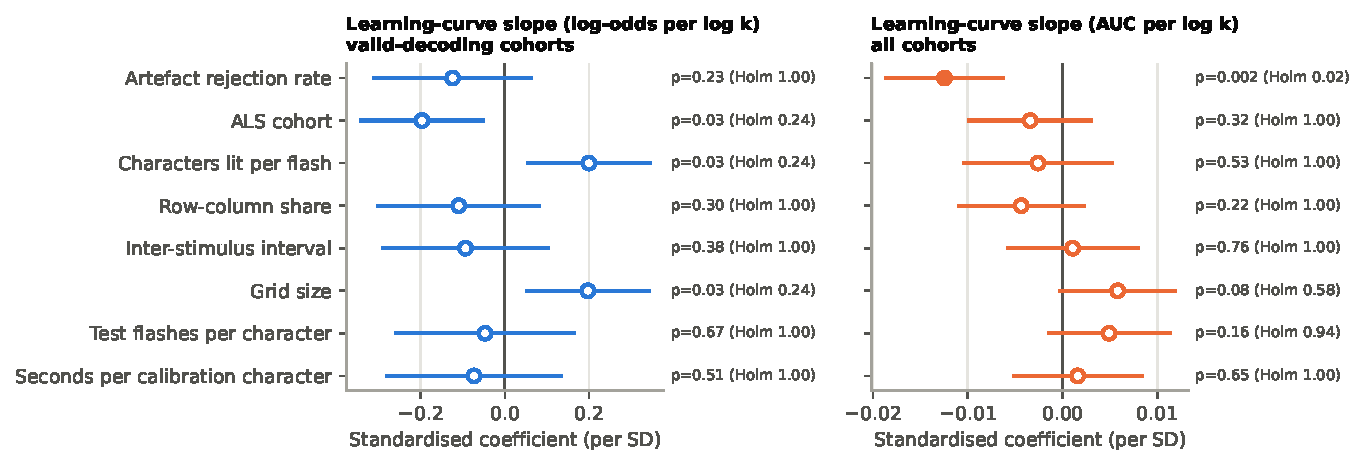
\includegraphics[width=0.92\textwidth]{fig3_moderators_paper.pdf}
\caption{Standardised meta-regression coefficients ($\pm$95\% CI) of cohort learning-curve slope on each descriptor. Filled: significant after Holm correction.}
\label{fig:mods}
\end{figure*}

\subsection{Learning curves differ between cohorts}
Accuracy rose with $k$ in every cohort, but at different rates and to different levels (Fig.~\ref{fig:curves}). In valid cohorts the pooled slope was 1.06 log-odds per $\log k$ (95\% CI 0.83--1.28), with between-cohort heterogeneity ($\tau=0.20$, $I^2=0.88$, $p<0.001$); the 95\% prediction interval for a new cohort was 0.55--1.56. Intercepts varied more ($\tau=0.98$, $I^2=0.96$). On AUC across all 14 cohorts the pooled slope was 0.067 per $\log k$ ($I^2=0.84$).

\subsection{Calibration budgets vary about 15-fold}
B80 ranged from 2 characters (S1) to 30 (Q) among the 7 valid cohorts that reached it, a 15-fold spread; A and N did not reach it. The AUC budget gave the same picture across all 14 cohorts, ranging from 2 to 30 characters (15-fold) among the 8 that reached it, and ranked cohorts similarly (Fig.~\ref{fig:budgets}). In time, the AUC budget ranged from 45\,s (S1) to 900\,s (B). Four dynamic-stopping cohorts (I, J, K, M) reached neither budget, even at an AUC threshold of 0.70.

\subsection{Protocol descriptors do not explain slope differences}
None of the pre-specified protocol descriptors was associated with learning-curve slope after Holm correction, so H3 was not supported (Fig.~\ref{fig:mods}). In the exploratory analysis, artefact rejection rate was associated with the AUC slope ($\beta=-0.012$ per SD, $p=0.002$, Holm $p=0.016$): cohorts with noisier calibration data learned more slowly. Because this descriptor was chosen after the primary moderators were tested, it should be read as a hypothesis for future work rather than a confirmed effect. In valid cohorts, grid size, characters lit per flash and ALS status each explained about 38\% of slope variance ($p\approx0.03$, Holm $p=0.24$). These descriptors are collinear, since the ALS cohorts also used 36-character grids, so they cannot be separated. Test length, inter-stimulus interval and row--column share were not associated with slope.

\subsection{Budgets do not transport}
Pooling all other cohorts' participants never produced a budget at which 80\% of them were usable, so the primary predictor was undefined for every withheld cohort: no single calibration length served 80\% of users across protocols. The median budget of the other cohorts missed the withheld AUC budget by at least two characters in all 14 cohorts (median error 12; Fig.~\ref{fig:loco}) and missed B80 by at least two characters in all 9 valid cohorts (median 13). It overestimated budgets for fast cohorts (R, S1, S2) and underestimated them for slow ones (A, B, Q).

\begin{figure}[!tb]
\centering
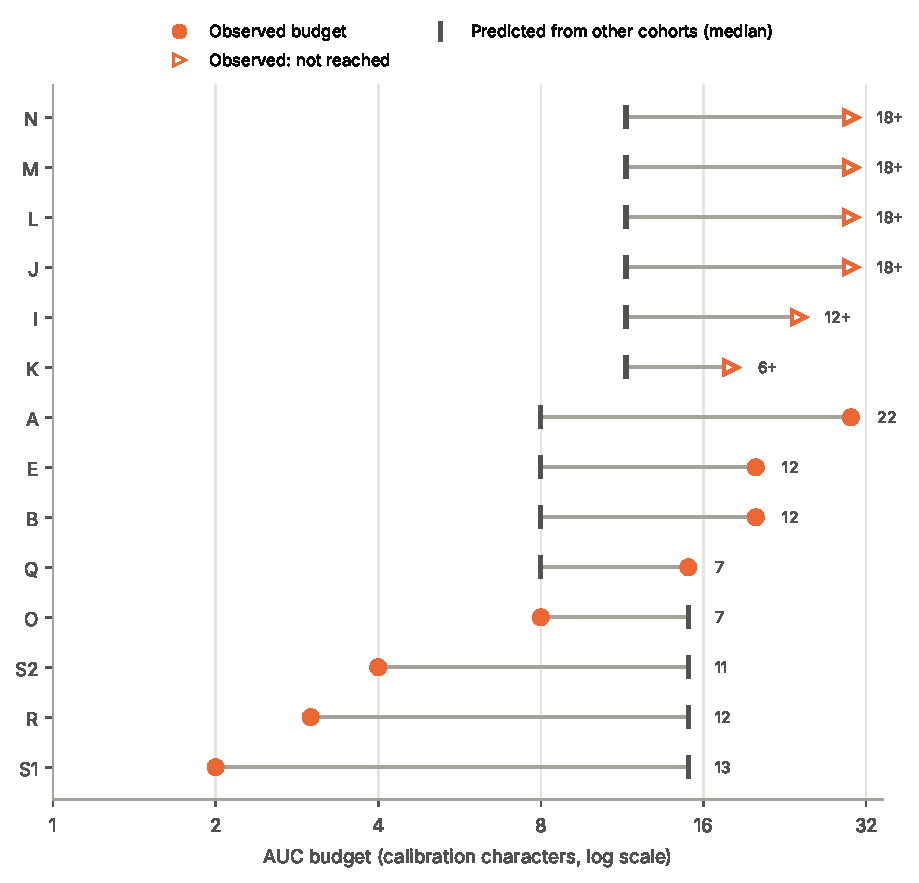
\includegraphics[width=\columnwidth]{fig4_transportability_paper.pdf}
\caption{Observed AUC budget per cohort (orange) versus the budget predicted from the other cohorts (tick); labels give the absolute error in characters (``+'': lower bound).}
\label{fig:loco}
\end{figure}

\subsection{Robustness}
The spread persisted in every variant (Table~\ref{tab:robust}). Removing high-artefact records let cohort N reach both budgets (B80 $=20$, AUC budget $=30$), consistent with the moderator result.

\begin{table}[!tb]
\centering
\caption{Budget across robustness variants: cohorts reached, range (characters), max/min ratio.}
\label{tab:robust}
\setlength{\tabcolsep}{3pt}
\footnotesize
\begin{tabular}{lcc}
\toprule
Variant & B80 & AUC budget\\
\midrule
Primary & 7/9, 2--30, 15$\times$ & 8/14, 2--30, 15$\times$\\
First session only & 7/9, 2--36, 18$\times$ & 7/14, 2--30, 15$\times$\\
$\leq$20\% artefacts & 8/9, 2--30, 15$\times$ & 9/14, 2--30, 15$\times$\\
Lower threshold$^a$ & 8/9, 2--25, 12.5$\times$ & 9/14, 2--20, 10$\times$\\
Higher threshold$^b$ & 5/9, 2--30, 15$\times$ & 5/14, 3--36, 12$\times$\\
\bottomrule
\multicolumn{3}{l}{\scriptsize $^a$accuracy 0.60 / AUC 0.70. $^b$accuracy 0.80 / AUC 0.80.}
\end{tabular}
\end{table}

\section{Discussion}
\subsection{Principal findings}
With one fixed decoder and one fixed rule, the calibration at which 80\% of users reached usable accuracy ranged from 2 to 30 characters, or from under a minute to 15 minutes. A budget estimated elsewhere was wrong by a median of 12--13 characters, and no single budget served 80\% of all participants.

\subsection{Implications}
For method papers, this means a claim such as ``60\% less calibration'' is relative to a baseline that itself differs severalfold between datasets; the same absolute saving can be decisive in a slow cohort and irrelevant in a fast one. Calibration-reduction methods should be evaluated on several cohorts with per-cohort budgets. For deployment, calibration lengths copied from the literature will over-calibrate users in fast settings and under-calibrate them in slow ones, so budgets should be set per protocol and site, or adaptively. The pre-specified protocol descriptors did not explain the spread. Exploratory evidence points to recording quality: artefact rate was associated with slower learning, and removing noisy records moved a cohort from censored to a finite budget. This needs confirmation in an independent sample, but reporting artefact rates alongside calibration results would already make budgets more comparable. This agrees with Gorenshtein et al., who found cohort-specific mappings only partly explained by protocol \cite{gorenshtein2026}.

\subsection{Limitations}
The analysis is offline with a fixed decoder rather than the original online classifier, whose BCI2000 parameters are not public. In five dynamic-stopping cohorts our decoder fell well below online accuracy, so B80 was restricted to valid cohorts and an AUC budget was added. Protocol, laboratory, hardware and population are nested within cohorts, so associations are not causal and ALS effects cannot be separated from grid size or timing. Cohorts with only 18 calibration characters censor larger budgets, so the true spread may exceed 15-fold. Finally, we tested one decoder; deep, transfer-learned or foundation-model decoders \cite{lawhern2018,wu2022,jiang2024} may lower budgets, and whether they remove between-cohort heterogeneity is left to future work.

\section{Conclusion}
Across 14 cohorts and 224 participants, the calibration budget for a fixed P300 decoder varied about 15-fold, and did not transport between cohorts. Pre-specified protocol descriptors did not explain this spread; exploratory analysis points to recording quality. Calibration-reduction studies should report per-cohort budgets, and deployments should set calibration per protocol and site. Code that reproduces all results from bigP3BCI v1.0.0, including the independent verification, is available at \url{https://github.com/<username>/p300-calibration-budget}.

\FloatBarrier
\begin{thebibliography}{99}
\bibitem{farwell1988} L.~A. Farwell and E.~Donchin, ``Talking off the top of your head: toward a mental prosthesis utilizing event-related brain potentials,'' \emph{Electroencephalogr. Clin. Neurophysiol.}, vol.~70, no.~6, pp.~510--523, 1988, doi:10.1016/0013-4694(88)90149-6.
\bibitem{sellers2006} E.~W. Sellers and E.~Donchin, ``A P300-based brain--computer interface: initial tests by ALS patients,'' \emph{Clin. Neurophysiol.}, vol.~117, no.~3, pp.~538--548, 2006, doi:10.1016/j.clinph.2005.06.027.
\bibitem{guger2009} C.~Guger, S.~Daban, E.~Sellers \emph{et al.}, ``How many people are able to control a P300-based brain--computer interface (BCI)?'' \emph{Neurosci. Lett.}, vol.~462, no.~1, pp.~94--98, 2009, doi:10.1016/j.neulet.2009.06.045.
\bibitem{hong2025} J.~Hong, G.~Mackellar, and S.~Ghane, ``SpellerSSL: Self-supervised learning with P300 aggregation for speller BCIs,'' in \emph{Proc. NeurIPS}, 2025, arXiv:2509.19401.
\bibitem{gao2023} W.~Gao, W.~Huang \emph{et al.}, ``Eliminating or shortening the calibration for a P300 brain--computer interface based on a convolutional neural network and big electroencephalography data: an online study,'' \emph{IEEE Trans. Neural Syst. Rehabil. Eng.}, 2023.
\bibitem{chen2026} S.~Chen \emph{et al.}, ``Adaptive semi-supervised training of P300 ERP-BCI speller system with minimum calibration effort,'' arXiv:2602.15955, 2026.
\bibitem{wu2022} D.~Wu, Y.~Xu, and B.-L. Lu, ``Transfer learning for EEG-based brain--computer interfaces: a review of progress made since 2016,'' \emph{IEEE Trans. Cogn. Dev. Syst.}, vol.~14, no.~1, pp.~4--19, 2022, doi:10.1109/TCDS.2020.3007453.
\bibitem{gorenshtein2026} A.~Gorenshtein, Y.~Adiniaev, T.~Liba, Y.~Barash, E.~Klang, and O.~Daniel, ``Calibration-derived decoder discriminability is associated with online P300-speller accuracy, but the fitted mapping does not transport across cohorts,'' \emph{medRxiv}, 2026, doi:10.64898/2026.07.30.26359353.
\bibitem{viering2023} T.~Viering and M.~Loog, ``The shape of learning curves: a review,'' \emph{IEEE Trans. Pattern Anal. Mach. Intell.}, vol.~45, no.~6, pp.~7799--7819, 2023, doi:10.1109/TPAMI.2022.3220744.
\bibitem{koh2021} P.~W. Koh, S.~Sagawa, H.~Marklund \emph{et al.}, ``WILDS: a benchmark of in-the-wild distribution shifts,'' in \emph{Proc. 38th Int. Conf. Mach. Learn. (ICML)}, PMLR vol.~139, pp.~5637--5664, 2021.
\bibitem{kilani2024} S.~Kilani, S.~N. Aghili, Y.~Fathi, and A.~I. Sburlea, ``Optimization of transfer learning based on source sample selection in Euclidean space for P300-based brain-computer interfaces,'' \emph{Front. Neurosci.}, 2024.
\bibitem{jiang2024} W.~Jiang, L.~Zhao, and B.-L. Lu, ``Large brain model for learning generic representations with tremendous EEG data in BCI,'' in \emph{Proc. Int. Conf. Learn. Represent. (ICLR)}, 2024.
\bibitem{moabb2024} S.~Chevallier \emph{et al.}, ``The largest EEG-based BCI reproducibility study for open science: the MOABB benchmark,'' arXiv:2404.15319, 2024.
\bibitem{song2024} M.~Song, D.~Gwon, S.~C. Jun, and M.~Ahn, ``Signal alignment for cross-datasets in P300 brain-computer interfaces,'' \emph{J. Neural Eng.}, vol.~21, no.~3, 036007, 2024, doi:10.1088/1741-2552/ad430d.
\bibitem{bianchi2022} L.~Bianchi, R.~Ferrante, Y.~Hu, G.~Sahonero-Alvarez, and N.~Z. Zenia, ``Merging brain-computer interface P300 speller datasets: perspectives and pitfalls,'' \emph{Front. Neuroergon.}, 2022.
\bibitem{mainsah2016} B.~O. Mainsah, L.~M. Collins, and C.~S. Throckmorton, ``Using the detectability index to predict P300 speller performance,'' \emph{J. Neural Eng.}, vol.~13, no.~6, 066007, 2016, doi:10.1088/1741-2560/13/6/066007.
\bibitem{bigp3bci} B.~Mainsah, C.~Fleeting, T.~Balmat, E.~Sellers, and L.~Collins, ``bigP3BCI: an open, diverse and machine learning ready P300-based brain-computer interface dataset (v1.0.0),'' PhysioNet, 2025, doi:10.13026/0byy-ry86.
\bibitem{schalk2004} G.~Schalk, D.~J. McFarland, T.~Hinterberger, N.~Birbaumer, and J.~R. Wolpaw, ``BCI2000: a general-purpose brain--computer interface (BCI) system,'' \emph{IEEE Trans. Biomed. Eng.}, vol.~51, no.~6, pp.~1034--1043, 2004, doi:10.1109/TBME.2004.827072.
\bibitem{townsend2010} G.~Townsend, B.~K. LaPallo, C.~B. Boulay \emph{et al.}, ``A novel P300-based brain--computer interface stimulus presentation paradigm: moving beyond rows and columns,'' \emph{Clin. Neurophysiol.}, vol.~121, no.~7, pp.~1109--1120, 2010, doi:10.1016/j.clinph.2010.01.030.
\bibitem{gramfort2013} A.~Gramfort, M.~Luessi, E.~Larson \emph{et al.}, ``MEG and EEG data analysis with MNE-Python,'' \emph{Front. Neurosci.}, vol.~7, 267, 2013, doi:10.3389/fnins.2013.00267.
\bibitem{virtanen2020} P.~Virtanen, R.~Gommers, T.~E. Oliphant \emph{et al.}, ``SciPy 1.0: fundamental algorithms for scientific computing in Python,'' \emph{Nat. Methods}, vol.~17, no.~3, pp.~261--272, 2020, doi:10.1038/s41592-019-0686-2.
\bibitem{pedregosa2011} F.~Pedregosa, G.~Varoquaux, A.~Gramfort \emph{et al.}, ``Scikit-learn: machine learning in Python,'' \emph{J. Mach. Learn. Res.}, vol.~12, pp.~2825--2830, 2011.
\bibitem{seabold2010} S.~Seabold and J.~Perktold, ``Statsmodels: econometric and statistical modeling with Python,'' in \emph{Proc. 9th Python in Science Conf.}, pp.~92--96, 2010, doi:10.25080/Majora-92bf1922-011.
\bibitem{blankertz2011} B.~Blankertz, S.~Lemm, M.~Treder, S.~Haufe, and K.-R. M\"{u}ller, ``Single-trial analysis and classification of ERP components---a tutorial,'' \emph{NeuroImage}, vol.~56, no.~2, pp.~814--825, 2011, doi:10.1016/j.neuroimage.2010.06.048.
\bibitem{ledoit2004} O.~Ledoit and M.~Wolf, ``A well-conditioned estimator for large-dimensional covariance matrices,'' \emph{J. Multivar. Anal.}, vol.~88, no.~2, pp.~365--411, 2004, doi:10.1016/S0047-259X(03)00096-4.
\bibitem{mainsah2015} B.~O. Mainsah, L.~M. Collins, K.~A. Colwell \emph{et al.}, ``Increasing BCI communication rates with dynamic stopping towards more practical use: an ALS study,'' \emph{J. Neural Eng.}, vol.~12, no.~1, 016013, 2015, doi:10.1088/1741-2560/12/1/016013.
\bibitem{dersimonian1986} R.~DerSimonian and N.~Laird, ``Meta-analysis in clinical trials,'' \emph{Control. Clin. Trials}, vol.~7, no.~3, pp.~177--188, 1986, doi:10.1016/0197-2456(86)90046-2.
\bibitem{higgins2002} J.~P.~T. Higgins and S.~G. Thompson, ``Quantifying heterogeneity in a meta-analysis,'' \emph{Stat. Med.}, vol.~21, no.~11, pp.~1539--1558, 2002, doi:10.1002/sim.1186.
\bibitem{knapp2003} G.~Knapp and J.~Hartung, ``Improved tests for a random effects meta-regression with a single covariate,'' \emph{Stat. Med.}, vol.~22, no.~17, pp.~2693--2710, 2003, doi:10.1002/sim.1482.
\bibitem{holm1979} S.~Holm, ``A simple sequentially rejective multiple test procedure,'' \emph{Scand. J. Stat.}, vol.~6, no.~2, pp.~65--70, 1979.
\bibitem{lawhern2018} V.~J. Lawhern, A.~J. Solon, N.~R. Waytowich, S.~M. Gordon, C.~P. Hung, and B.~J. Lance, ``EEGNet: a compact convolutional neural network for EEG-based brain--computer interfaces,'' \emph{J. Neural Eng.}, vol.~15, no.~5, 056013, 2018, doi:10.1088/1741-2552/aace8c.
\end{thebibliography}

\end{document}
